\documentclass[12pt,english,dvipsnames,aspectratio=169,handout]{beamer}\usepackage[]{graphicx}\usepackage[]{xcolor}
% maxwidth is the original width if it is less than linewidth
% otherwise use linewidth (to make sure the graphics do not exceed the margin)
\makeatletter
\def\maxwidth{ %
  \ifdim\Gin@nat@width>\linewidth
    \linewidth
  \else
    \Gin@nat@width
  \fi
}
\makeatother

\definecolor{fgcolor}{rgb}{0.345, 0.345, 0.345}
\newcommand{\hlnum}[1]{\textcolor[rgb]{0.686,0.059,0.569}{#1}}%
\newcommand{\hlstr}[1]{\textcolor[rgb]{0.192,0.494,0.8}{#1}}%
\newcommand{\hlcom}[1]{\textcolor[rgb]{0.678,0.584,0.686}{\textit{#1}}}%
\newcommand{\hlopt}[1]{\textcolor[rgb]{0,0,0}{#1}}%
\newcommand{\hlstd}[1]{\textcolor[rgb]{0.345,0.345,0.345}{#1}}%
\newcommand{\hlkwa}[1]{\textcolor[rgb]{0.161,0.373,0.58}{\textbf{#1}}}%
\newcommand{\hlkwb}[1]{\textcolor[rgb]{0.69,0.353,0.396}{#1}}%
\newcommand{\hlkwc}[1]{\textcolor[rgb]{0.333,0.667,0.333}{#1}}%
\newcommand{\hlkwd}[1]{\textcolor[rgb]{0.737,0.353,0.396}{\textbf{#1}}}%
\let\hlipl\hlkwb

\usepackage{framed}
\makeatletter
\newenvironment{kframe}{%
 \def\at@end@of@kframe{}%
 \ifinner\ifhmode%
  \def\at@end@of@kframe{\end{minipage}}%
  \begin{minipage}{\columnwidth}%
 \fi\fi%
 \def\FrameCommand##1{\hskip\@totalleftmargin \hskip-\fboxsep
 \colorbox{shadecolor}{##1}\hskip-\fboxsep
     % There is no \\@totalrightmargin, so:
     \hskip-\linewidth \hskip-\@totalleftmargin \hskip\columnwidth}%
 \MakeFramed {\advance\hsize-\width
   \@totalleftmargin\z@ \linewidth\hsize
   \@setminipage}}%
 {\par\unskip\endMakeFramed%
 \at@end@of@kframe}
\makeatother

\definecolor{shadecolor}{rgb}{.97, .97, .97}
\definecolor{messagecolor}{rgb}{0, 0, 0}
\definecolor{warningcolor}{rgb}{1, 0, 1}
\definecolor{errorcolor}{rgb}{1, 0, 0}
\newenvironment{knitrout}{}{} % an empty environment to be redefined in TeX

\usepackage{alltt}
\usepackage{fontspec}
\setsansfont[Mapping=tex-text]{Fira Sans}
\setcounter{secnumdepth}{4}
\setcounter{tocdepth}{4}
\usepackage[normalem]{ulem}
\usepackage[T1]{fontenc}
\usepackage{dcolumn}
\usepackage{booktabs}
\usepackage{bm}
\usepackage{setspace}
\makeatletter
\usetheme{metropolis}
\setbeamertemplate{frame footer}{Bosancianu | Schaub | Hertie School}
\setbeamerfont{page number in head/foot}{size=\tiny}
\setbeamercolor{footline}{fg=gray}
\usepackage{xcolor}
\setbeamercovered{transparent}
\usepackage{tikz}
\usetikzlibrary{arrows, positioning}
\usepackage[labelformat=empty]{caption}
% For table captions in Beamer
\usepackage[sectionbib]{apacite}
\renewcommand{\bibliographytypesize}{\footnotesize}
\makeatletter
\let\st@rtbibsection\@bibnewpage
\let\st@rtbibchapter\@bibnewpage
\makeatother
\usepackage{amsmath, mathtools}
\usepackage{xunicode}
\usepackage{hyperref}
\graphicspath{{./figures/}} 
% Defines a checkmark
\def\checkmark{\tikz\fill[scale=0.4,color=orange](0,.35) -- (.25,0) -- (1,.7) -- (.25,.15) -- cycle;}
% wide itemize and enumerate
\newenvironment{wideitemize}{\itemize\addtolength{\itemsep}{.3em}}{\enditemize}
\newenvironment{wideenumerate}{\enumerate\addtolength{\itemsep}{.3em}}{\endenumerate}
% boxes
\def\boxitorange#1{%
  \smash{\color{orange}\fboxrule=1pt\relax\fboxsep=2pt\relax%
  \llap{\rlap{\fbox{\vphantom{0}\makebox[#1]{}}}~}}\ignorespaces
}
\def\boxitblue#1{%
  \smash{\color{blue}\fboxrule=1pt\relax\fboxsep=2pt\relax%
  \llap{\rlap{\fbox{\vphantom{0}\makebox[#1]{}}}~}}\ignorespaces
}
\newcommand{\indep}{\perp \!\!\!\! \perp}
\setbeamertemplate{itemize items}{\checkmark}
\usepackage{multirow}
\hypersetup{pdfauthor={Bosancianu and Schaub},
	pdftitle={Statistical Modeling and Causal Inference with R},
	pdfsubject={Week 5: Instrumental variable estimation},
	pdfkeywords={Berlin, Hertie, 2020, week 5}}
\title{\textsc{Statistical Modeling and Causal Inference with R}}
\subtitle{Week 5: Instrumental variable estimation}
\date{October 5, 2020}
\author{Manuel Bosancianu \hfill Max Schaub}
\institute{Hertie School of Governance}
\IfFileExists{upquote.sty}{\usepackage{upquote}}{}
\begin{document}
\maketitle


\begin{frame}
	\frametitle{Today's focus}
	\begin{itemize}
		\item Why instrumental variables? An example.
		\item Defining instrumental variables
		\item Analyze experiments affected by non-compliance using IVs
		\item Use of IVs in observational studies
	\end{itemize}
\end{frame}


\section{Why instrumental variables? An example.}

\begin{frame}
  \frametitle{Why instrumental variables? An example.}
  Example: Estimate effect of internet use on right-wing support \cite{schaub_voter_2020}.
	\begin{itemize} \scriptsize
		\item Rise of right-wing populism coincides with internet age
		\item Internet way for right-wing actors to circumvent gatekeepers in media
		\item Targeted online campaigns during election time
	\end {itemize}
	 \begin{figure} 
    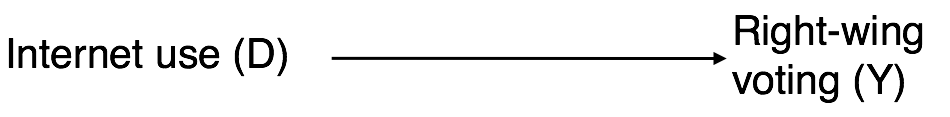
\includegraphics[height=.07\textheight,keepaspectratio=true]{../04-figures/05/01-w5_dag_1.png}
    \end{figure}
\end{frame}


\begin{frame}
  \frametitle{Why instrumental variables? An example.}
  The problem is tht there are many plausible confounders, some of them observable\ldots
	\begin{itemize} \scriptsize
		\item Education (educated use internet more, vote less often for right)
		\item Age (young use internet more, vote more often for right)
		\item \ldots
	\end {itemize}
	 \begin{figure} 
    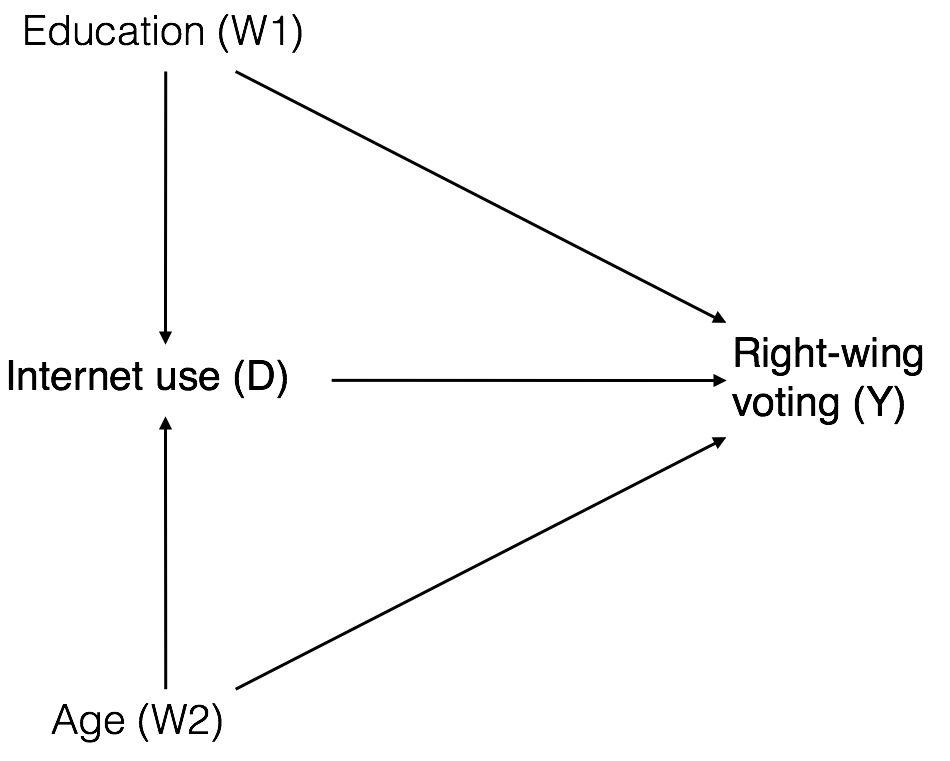
\includegraphics[height=.45\textheight,keepaspectratio=true]{../04-figures/05/02-w5_dag_2.png}
    \end{figure}
\end{frame}


\begin{frame}
  \frametitle{Why instrumental variables? An example.}
  Observable confounders can be controlled for by conditioning on them\ldots
	 \begin{figure} 
    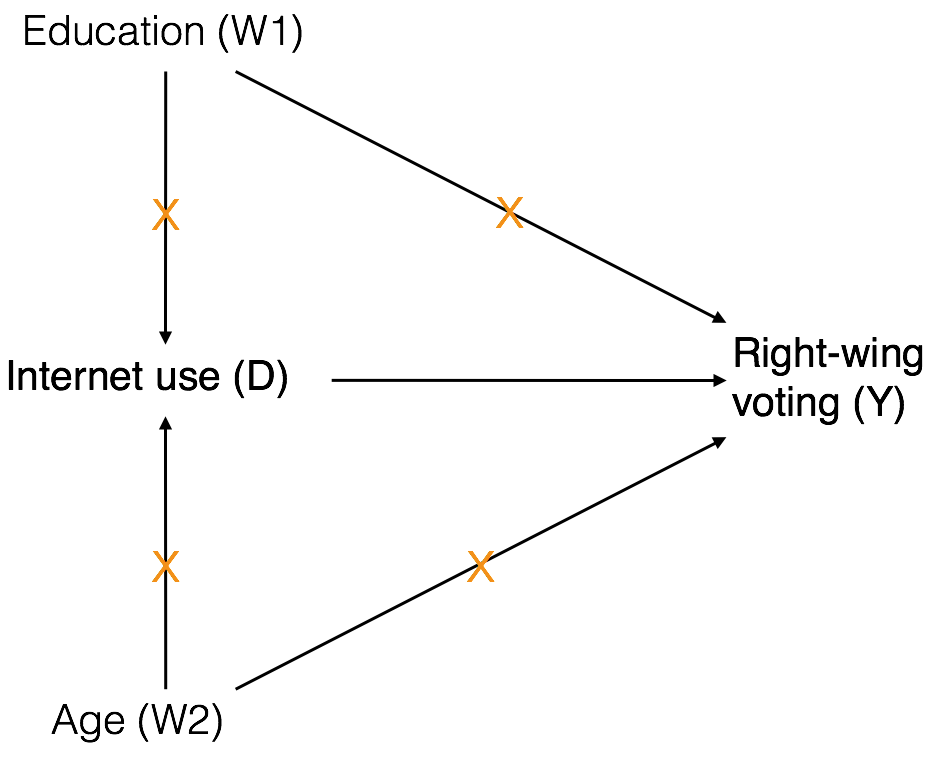
\includegraphics[height=.45\textheight,keepaspectratio=true]{../04-figures/05/03-w5_dag_3.png}
    \end{figure}
\vspace{3cm}
\end{frame}

\begin{frame}
  \frametitle{Why instrumental variables? An example.}
\ldots but this is impossible for unobservable confounders, e.g.\ right-wing mindset!
	\begin{itemize} \scriptsize
		\item Right-wing ideology predicts right-wing voting, and plausibly also lets people seek out right-wing content online, leading to higher internet consumption
	\end {itemize}
	\begin{figure} 
    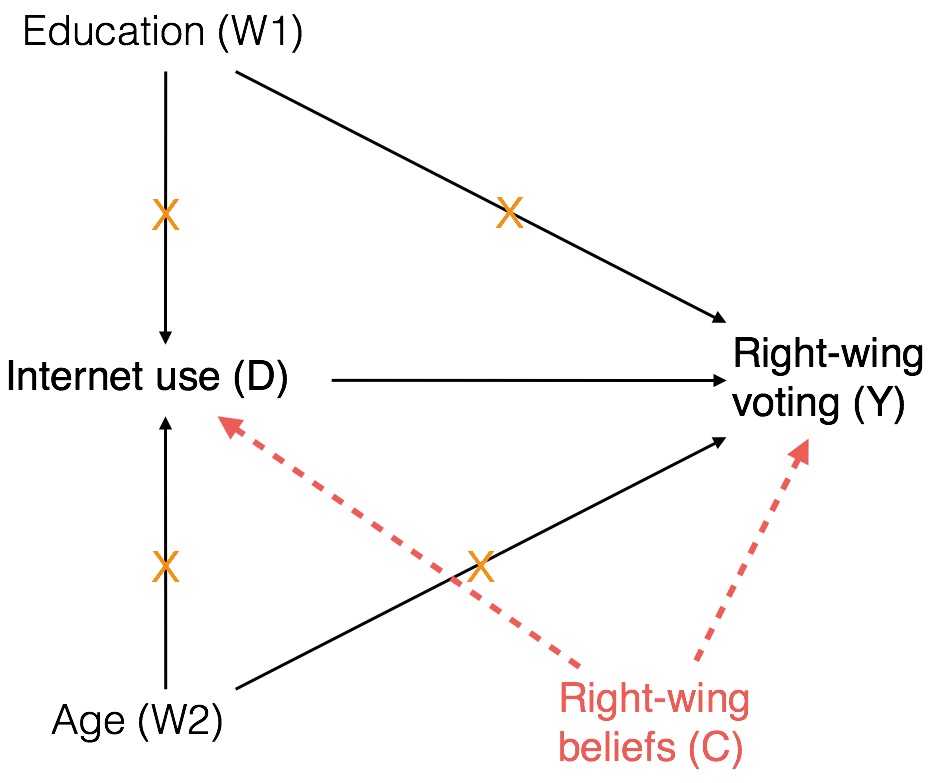
\includegraphics[height=.45\textheight,keepaspectratio=true]{../04-figures/05/04-w5_dag_4.png}
    \end{figure}
\vspace{3cm}
\end{frame}


\begin{frame}
  \frametitle{Why instrumental variables? An example.}
  \footnotesize 
  We solve this problem with an instrumental variable: a variable that changes the endogenous predictor internet use -- and therefore the outcome -- but is unrelated to possible confounders, esp.\ right-wing beliefs. 
  
  Here, local broadband availability is used as such an instrument:
	 \begin{figure} 
    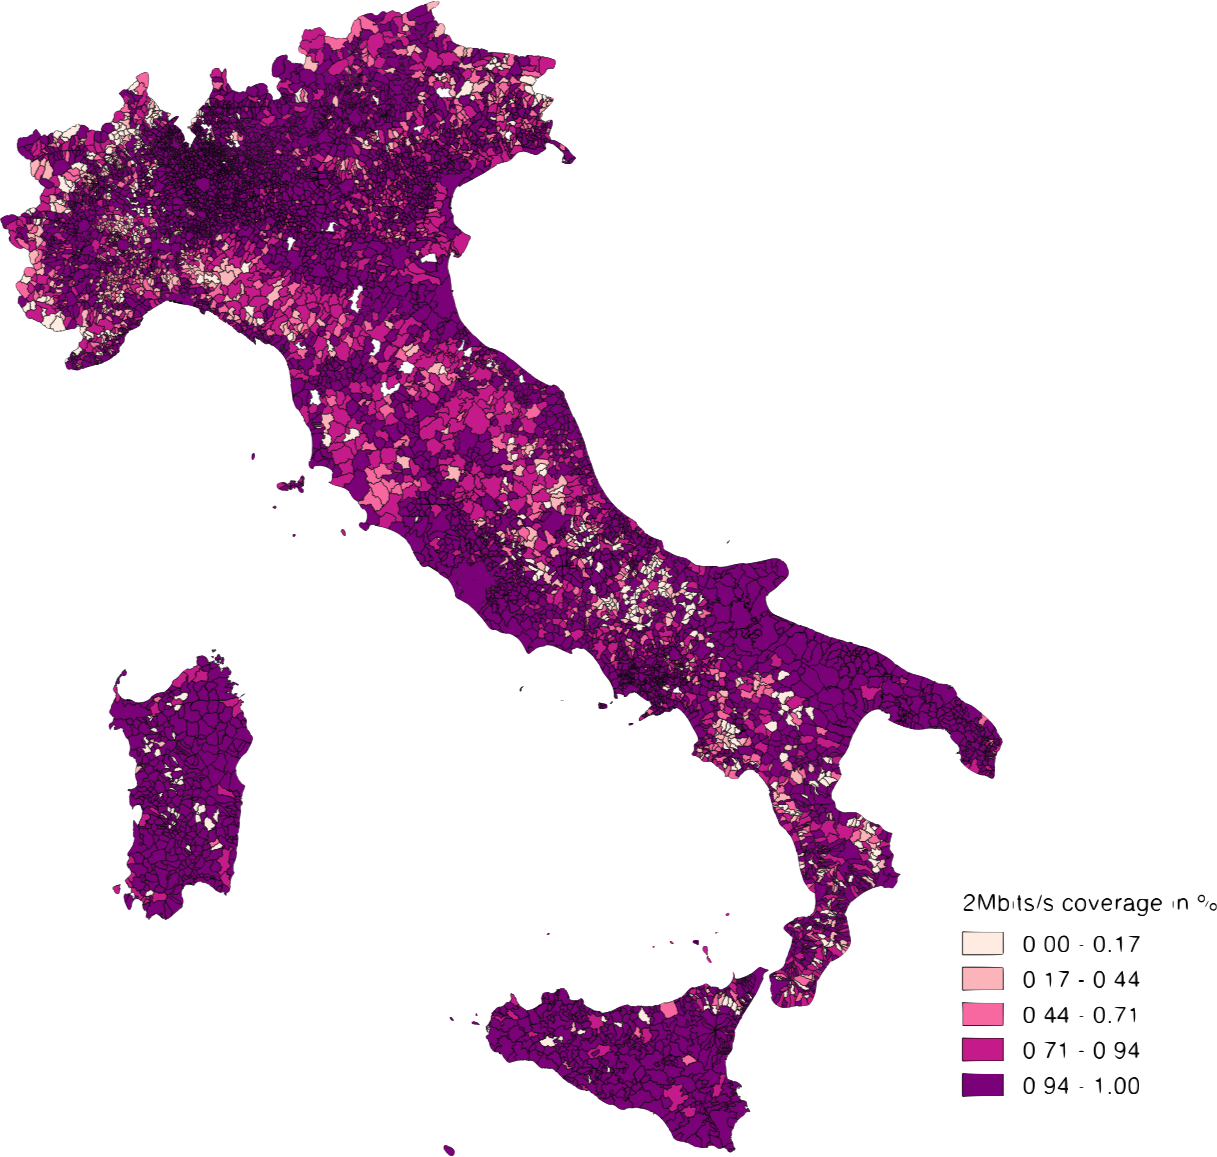
\includegraphics[height=.55\textheight, keepaspectratio=true]{../04-figures/05/07-bbcoverage_italy}
    \end{figure}
\end{frame}


\begin{frame}
  \frametitle{Why instrumental variables? An example.}
  Justification for relevance of the instrument and independence of confounders:
	\begin{itemize} \footnotesize 
		\item The availability of high-speed internet increases internet consumption, and makes possible the delivery of higher quality, more interesting, and more persuasive content. 
		\item At the same time, broadband availability is unlikely to be correlated with right-wing voting through any other channel than increasing internet use, given some controls such as economic prowess of the region and population density/degree of urbanization. 
		\item In particular, it is only implausibly correlated with right-wing ideology.
	\end {itemize}
\vspace{3cm}
\end{frame}


\begin{frame}
  \frametitle{Why instrumental variables? An example.}
    In the DAG, this IV appears as a variable that is causally connected to internet use, but shares no open paths with the potential confounders.
	\begin{figure} 
    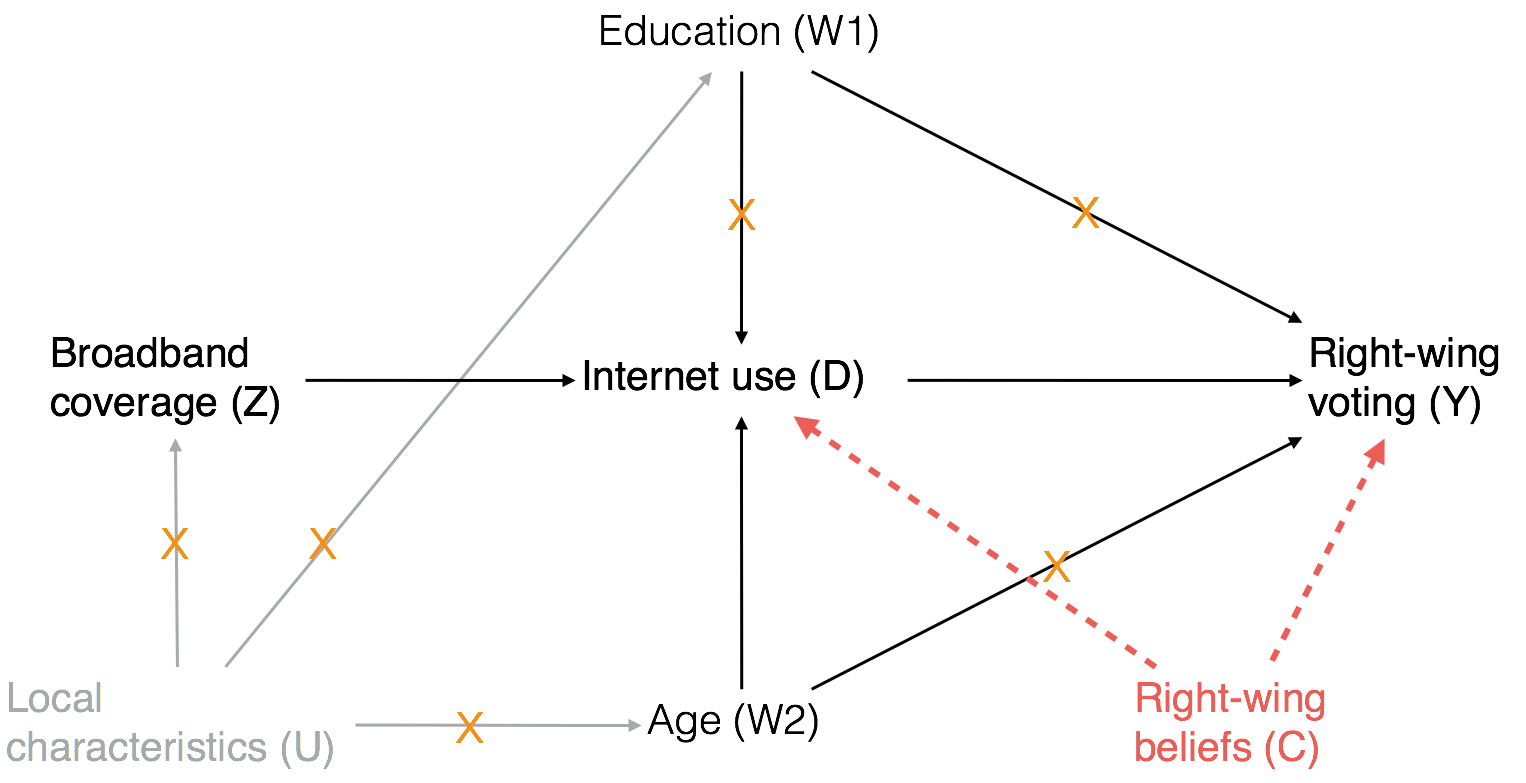
\includegraphics[height=.45\textheight,keepaspectratio=true]{../04-figures/05/05-w5_dag_5.png}
    \end{figure}
\vspace{3cm}
\end{frame}



\section{Defining instrumental variables}

\begin{frame}
  \frametitle{Defining IVs: Basic idea}
    We are interested in the causal effect of $D$ on $Y$, but the relationship is subject to confounding, measurement problems, or non-compliance. \\
    \vspace{3mm}
    Basic idea of instrumental variables (IV): \\ 
    Split the variation of $D$ into two parts
  \begin{itemize} \footnotesize
  	\item one potentially related to (potentially unobserved) confounders $W$
	  \item one truly exogenous, i.e.\ caused by other factors unrelated to the confounders
	  \item To find the portion of $D$ unrelated to confounders, one needs a variable $Z$ (the \textcolor{orange}{instrumental variable}) that is (as if) randomly assigned and related to $D$
  \end{itemize}
\end{frame}



\begin{frame}
  \frametitle{Defining IVs through their requirements}
  An instrumental variable (Z) is a variable that:
  \begin{enumerate} 
		\item Is substantially related to the treatment/independent variable (D) $\rightarrow$ the \textcolor{orange}{first stage}\\
		
		\scriptsize The first stage is shown with a positive correlation between D and Z \normalsize
		
		\item Only influences the outcome Y through its effect on D, i.e.\ there are no other causal paths running from Z to Y other than through D $\rightarrow$ the \textcolor{orange}{exclusion restriction}. \\
	  	
	  	\scriptsize The exclusion restriction is not fully testable, but it implies that:
		  \begin{itemize} \scriptsize
		    \item Z is not correlated with any confounder influencing the relationship between the treatment/independent variable (D) and the outcome (Y).
		    \item Z should not predict treatments or outcomes similar to D or Y (placebo/falsification criterion).
	    \end {itemize}
	\end {enumerate}
\end{frame}



\begin{frame}
  \frametitle{Defining IVs as DAG}
  An instrumental variable (Z) is a variable that:
	\begin{enumerate} 
		\item Is connected through a single causal path to the endogenous predictor D
		\item Is not a descendant of any confounder (W1, W2, etc.\ )
	\end {enumerate}
	\begin{figure} 
    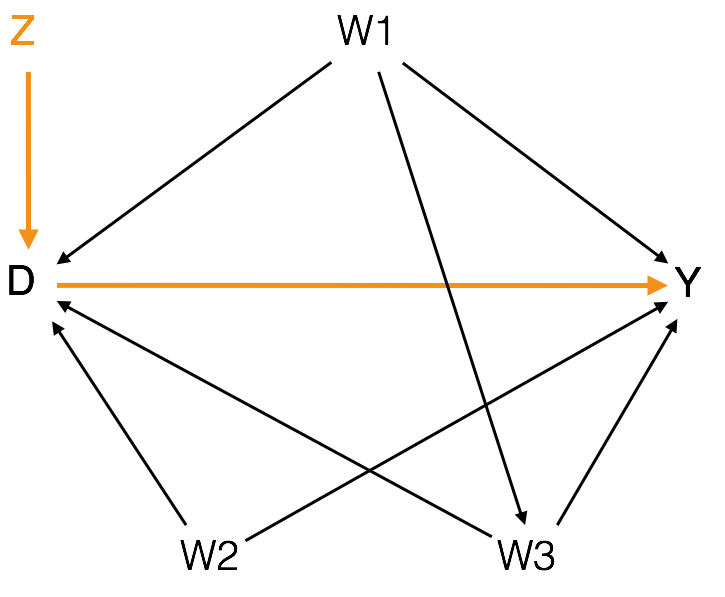
\includegraphics[height=.45\textheight,keepaspectratio=true]{../04-figures/05/06-w5_dag_6.png}
    \end{figure}
\end{frame}



\begin{frame}
  \frametitle{Defining IVs in the POF}
The basic setup for IVs in the potential outcomes framework:\\ \footnotesize
    \vspace{3mm}
    The instrument/(randomized) treatment assignment: $Z_i$  \\
    The potential treatment variables: $D_{i}|Z_{i} = 1$ and $D_{i}|Z_{i} = 0$
  \begin{enumerate} \footnotesize
  	\item $D_{i}|Z_i=1$: treatment status if assigned to treatment
	 \item $D_{i}|Z_i=0$: treatment status if not assigned to treatment
  \end{enumerate}
    The potential outcomes: $[Y_i = Y_i|Z_i=z,D_i=d]$ \\ 
    with $z \in \{0,1\}$ and $d \in \{0,1\}$  \\
    \vspace{3cm}
\end{frame}



\begin{frame}
  \frametitle{Defining IVs in the POF}
Based on the POF notation, we can define several \textcolor{orange}{quantities of interest}:\\
    \vspace{3mm}
  \begin{table}\footnotesize
  \begin{tabular}{ll} 
    The first stage:    & $E[D_i|Z_i=1]-E[D_i|Z_i=0]$ \\
    The reduced form:   & $E[Y_i|Z_i=1]-E[Y_i|Z_i=0]=ITT$ \\
    \rule{0pt}{5ex}   
    The Wald estimator: &$\cfrac{E[Y_i|Z_I=1]-E[Y_i|Z_I=0]}{E[D_i|Z_I=1]-E[D_i|Z_I=0]}=LATE$\\
  \end{tabular}
  \end{table}

\scriptsize 
\textbf{First stage}: the effect of Z on D/the share of individuals $i$ that \emph{comply}, i.e.\ who change their treatment status if assigned to the treatment.  \\ 
\textbf{Reduced form/ intent-to-treat (ITT) effect}: effect of being assigned to the treatment, estimates the encouragement or program effect; causally identified because randomly assigned, but unlike ATE in case of partial compliance (a first-stage<1)\\
\textbf{Wald estimator}: the ITT scaled up by the first-stage, estimates the local average treatment effect (LATE) under certain assumptions
\end{frame}



\begin{frame}
  \frametitle{IV assumptions} 
The POF notation also allows us to state \textcolor{orange}{assumptions} invoked by IV analyses more formally:\\
  \begin{itemize} \footnotesize
    \item Relevance/first stage: $Z{\not\!\perp\!\!\!\perp}D$ \\
    \item Exclusion restriction:  $Z{\perp\!\!\!\perp}W$ and $Z{\perp\!\!\!\perp}\!Y|D,W$ \\
    \item Stable Unit Treatment Assumption (SUTVA): no spillovers between treated and untreated units \\
    \item Monotonicity: Effect of treatment only in one direction (either positive or negative) \\
    \item Homogeneity: Constant treatment effect assumption
  \end{itemize}
  \vspace{3cm}
\end{frame}




\begin{frame}
  \frametitle{Defining IVs in the POF}
  Distinguishing between treatment assignment Z and actual treatment received also allows us to define four \textcolor{orange}{principle strata} or \textcolor{orange}{compliance types} :\\
    \vspace{3mm}
  \begin{itemize} \scriptsize
  	\item compliers: $[D_i|Z_i=1] = 1$ and $[D_i|Z_i=0]=0$ 
    \item non-compliers $\left\{\def\arraystretch{1.2}\begin{tabular}{@{}l@{\quad}l@{}}
       always-takers: & $[D_i|Z_i=1] = [D_i|Z_i=0] = 1$\\
       never-takers:  & $[D_i|Z_i=1] = [D_i|Z_i=0] = 0$\\
       defiers:        & $[D_i|Z_i=1] = 0$ and $[D_i|Z_i=0] = 1$ 
\end{tabular}\right.$
  \end{itemize} \scriptsize
  \vspace{3cm}
\end{frame}



\begin{frame}
  \frametitle{Main uses of instrumental variables}
  Two main uses for instrumental variables:
  \begin{enumerate} \footnotesize 
		\item Analyze experiments affected by non-compliance 
		\item Make causal estimates for relationships affected by unmeasured or unmeasurable confounders in observational studies -- by exploiting natural experiments (cp.\ the example in the beginning)
	\end {enumerate}
  \vspace{3cm}
\end{frame}


\section{Analyze experiments affected by non-compliance using IVs}

\begin{frame}
\frametitle{Experiments with non-compliance}
\footnotesize
Example: micro-finance experiment, where 100 individuals each were assigned to treatment and control. \\
In a perfect world, this would look as follows:

\begin{table}\footnotesize
\begin{tabular}{lccc}
\hline
                                 & Assigned to control     & Assigned to treatment \\
                                 & $Z_i=0$                 & $Z_i=1$ \\ 
      \hline
     Did not take loan $D_i=0$   & \textcolor{orange}{100} & --                      \\
     Took out loan $D_i=1$       & --                      & \textcolor{orange}{100} \\
\hline
\end{tabular}
\caption{\scriptsize Observed treatment strata in perfect micro-finance experiment}
\end{table}

\vspace{-2mm}
\footnotesize All individuals would be compliers: those assigned to treatment took out loan, those assigned to control did not, i.e.\ $D_i=Z_i$. \\
Given random assignment, we could therefore calculate $NATE=ATE=ITT=E[Y_{i}|D_i=1] - E[Y_{i}|D_i=0]=E[Y_{i}|Z_i=1] - E[Y_{i}|Z_i=0]$
\end{frame}


\begin{frame}
\frametitle{Experiments with non-compliance}
\footnotesize
In the real world, experiments are often affected by imperfect compliance: some people might fail or refuse to take up the treatment, while others might `consume' it anyway. The data from a real-world experiment might therefore look as follows: \\
\begin{table}\centering\footnotesize
\begin{tabular}{lccc}
\hline
                                 & Assigned to control     & Assigned to treatment \\
                                 & $Z_i=0$                 & $Z_i=1$ \\ 
      \hline
     Did not take loan $D_i=0$   & \textcolor{orange}{80} & \textcolor{orange}{10} \\
     Took out loan $D_i=1$       & \textcolor{orange}{20}& \textcolor{orange}{90} \\
\hline
\end{tabular}
\caption{\scriptsize Observed treatment strata in real-world micro-finance experiment}
\end{table}

\vspace{-3mm}
\footnotesize With such selective non-compliance $NATE \neq ATE$ because potential outcomes of compliers might differ from those of non-compliers, i.e.\  $E[Y_{i0}|D = 1] - E[Y_{i0}|D = 0] \equiv E[u_i|D_i] \neq 0$.
\end{frame}



\begin{frame}
\frametitle{Recovering causal effects under non-compliance}
What can be done? What estimators can we recover?

\begin{enumerate} \footnotesize
  \item The Intent to Treat (ITT) effect: \\ $ITT=E[Y_{i}|Z_i=1] - E[Y_{i}|Z_i=0]$\\ \vspace{1mm}\scriptsize
  First, with random treatment assignment, we can always recover the ITT (sometimes also called encouragment or program effect), no matter whether treatment was received or not. Note: This can be useful for policy advice, assuming that non-compliance is part of all policy implementations. \footnotesize \vspace{1mm}

  \item  The local average treatment effect (LATE) for the compliers:\\
  $LATE=\cfrac{E[Y_i|Z_I=1]-E[Y_i|Z_I=0]}{E[D_i|Z_I=1]-E[D_i|Z_I=0]}$\\ \vspace{1mm}\scriptsize
  We may also recover the LATE (sometimes also called Complier Average Causal Effect (CACE), i.e.\ the causal effect of the treatment for the compliers only. 
  \end{enumerate}
\end{frame}



\begin{frame}
\frametitle{Recovering causal effects under non-compliance}
\footnotesize
However, for the LATE to be estimable we have to invoke the monotonicity and exclusion restrictions introduced above. Why is that so? \\
\vspace{2mm}
The problem: instead of the principal strata, which would allow us to identify the compliers, we can only ever see the observed strata, where different compliance types may mix. 

So instead of observing the principal strata:

\begin{table}\centering\footnotesize
\begin{tabular}{cccc}
\hline
                         &         & \multicolumn{2}{c}{$Z_i=0$} \\
                         &         & $D_i=1$      & $D_i=0$ \\ 
\hline
\multirow{2}{*}{$Z_i=1$} & $D_i=0$ & Defier                   & Never-taker \\
                         & $D_i=1$ & Always-taker       &  Complier  \\
\hline
\end{tabular}
\caption{\scriptsize Principal strata/compliance types}
\end{table}
\end{frame}


\begin{frame}
\frametitle{Recovering causal effects under non-compliance}
\footnotesize
We only ever see the observed strata, where different compliance types may mix:

\begin{table}[htbp]\centering\footnotesize
\begin{tabular}{cccc}
\hline
        &         $Z_i=0$         & $Z_i=1$ \\ 
\hline
$D_i=0$ & Complier/Never-taker  & Never-taker/Defier \\
$D_i=1$ & Always-taker/Defier   & Complier/Always-taker  \\
\hline
\end{tabular}
\caption{\scriptsize Observable treatment responses among subjects}
\end{table}
\end{frame}



\begin{frame}
\frametitle{Recovering causal effects under non-compliance}
\footnotesize
By invoking the montonicity assumption -- the assuption that assignment to treatment \emph{never dissuades} someone from taking the treatment -- we can `assume away' defiers:

\begin{table}[htbp]\centering\footnotesize
\begin{tabular}{cccc}
\hline
        &         $Z_i=0$         & $Z_i=1$ \\ 
\hline
$D_i=0$ & Complier/Never-taker  & Never-taker/\sout{Defier} \\
$D_i=1$ & Always-taker/\sout{Defier}   & Complier/Always-taker  \\
\hline
\end{tabular}
\end{table}

Our observed strata are now composed of individuals who either are unreactive to the treatment (always-takers and never-takers) or change their behavior in a consistent way in reaction to the treatment, and to treatment only -- the exclusion restriction. 
\end{frame}



\begin{frame}
\frametitle{Recovering causal effects under non-compliance}
\footnotesize Another way of conceiving the problem is that the ITT consists of four subgroups, corresponding to the principal strata and occuring with a certain probability $Pr$:
\begin{align*} \scriptsize
\text{ITT} &= \text{ITT}_{c} \times \text{Pr(compliers)} + \text{ITT}_{a} \times \text{Pr(always-takers)} \\
 &~~~ +  \text{ITT}_{n} \times \text{Pr(never-takers)} + \text{ITT}_{d} \times \text{Pr(defiers)} \\
 \shortintertext{\footnotesize Under monotonicity and the exclusion restriction, this simplifies to:}
\text{ITT} &= \text{ITT}_{c} \times \text{Pr(compliers)} + \text{ITT}_{a} \times \text{Pr(always-takers)} \\
 &~~~ +  \text{ITT}_{n} \times \text{Pr(never-takers)} + 0 \;\;[\text{\textbf{monotonicity}}] \\ 
 &= \text{ITT}_{c} \times \text{Pr(compliers)} +0 \times \text{Pr(always-takers)} \\
 &~~~ + 0 \times \text{Pr(never-takers)}\;\;[\text{\textbf{exclusion restriction}}] \\ 
 &= \text{ITT}_{c} \times \text{Pr(compliers)}\;\;[\text{\textbf{rearrange}}] \\ 
 \text{ITT}_{c} &=  \frac{\text{ITT}}{\text{Pr(compliers)}} = \text{LATE} \\
\end{align*}
\end{frame}


\begin{frame}
\frametitle{Recovering causal effects under non-compliance}
\footnotesize
Sometimes, we know that strictly only units assigned to treatment could get access to the treatment, e.g.\ in medical trials, where the administration of a new drug was confined to a controlled setting (but be mindful that these settings are rare).\\
\vspace{2mm}

In these cases, the situation simplifies, because we \emph{know} that there are no always-takers. Our uncertainty with regard to the observed strata is therefore reduced to the question who are compliers, and who are never-takers:

\begin{table}[htbp]\centering\footnotesize
\begin{tabular}{cccc}
\hline
        &         $Z_i=0$         & $Z_i=1$ \\ 
\hline
$D_i=0$ & Complier/Never-taker  & Never-taker/\sout{Defier} \\
$D_i=1$ & \sout{Always-taker}/\sout{Defier}   & Complier/\sout{Always-taker}  \\
\hline
\end{tabular}
\end{table}
In this case, our Wald/LATE estimator therefore recovers the average-treatment effect for the treated, the ATT! 
\end{frame}


\section{Estimating ITT and LATE in practice}

\begin{frame}
\frametitle{Estimating ITT and LATE in practice}
How to calculate ITT and LATE?\\
\vspace{2mm}
\footnotesize Given information on a) the frequency of observations, and b) the outcomes in each observed strata, and invoking our assumptions, we can estimate the ITT and LATE `by hand' as follows:
\begin{table}\centering\scriptsize
\begin{tabular}{lcccc}
\hline
Observed obs in treatment strata &    & $Z_i=0$                 & $Z_i=1$ \\ 
      \hline
&     $D_i=0$   & \textcolor{orange}{80} & \textcolor{orange}{10} \\
&     $D_i=1$       & \textcolor{orange}{20}& \textcolor{orange}{90} \\
\hline
\hline
Observed outcomes $E[Y_i|D_i,Z_i]$ &                                 & $Z_i=0$                 & $Z_i=1$ \\ 
      \hline
&     $D_i=0$   & \textcolor{orange}{500} & \textcolor{orange}{1000} \\
&     $D_i=1$       & \textcolor{orange}{450}& \textcolor{orange}{800} \\
\hline
\end{tabular}
\end{table}
\vspace{-3mm}
\scriptsize 
ITT = $E[Y_{i}|Z_i=1] - E[Y_{i}|Z_i=0] = (1000\times 0.1+800\times 0.9) - (500*0.8+450\times 0.2) = 330$ \\
First stage = $E[D_i|Z_i=1]-E[D_i|Z_i=0] = 90/(10+90) - 20/(20+80) = 0.7$ \\
LATE/Wald estimator = ITT/First stage = $330/0.7=471$
\end{frame}



\begin{frame}
\frametitle{Estimating ITT and LATE in practice}
\footnotesize
Instead of calculating the first-stage and LATE by hand, this can be done within the regression framework with a sequence of two regressions that define the two-stage-least-square estimator (abbreviated as 2SLS or TSLS):\\

\begin{enumerate} \footnotesize
  \item Calculate the first stage by regressing the treatment status on the treatment assigment:\\
   $D = \gamma_0 + \gamma_1 Z_i + v_i$ 
  \item Calculate the predicted values $\hat{D}$
  \item Regress the outcome Y on the predicted values $\hat{D}$: \\
   $Y_i = \beta_0 + \beta^{2sls} \hat{D} + u_i\;\;\;\;$ $\beta^{2sls}$ is the LATE estimator!\\
\end{enumerate}

The ITT/reduced form is simply:\\
$Y_i = \theta_0 + \theta_1 Z_i + w_i$ \\ \vspace{2mm}
\scriptsize The estimate for $\beta^{2sls}$ can also be obtained by $\frac{\theta_1}{\gamma_1}$.
\end{frame}


\begin{frame}
\frametitle{Estimating ITT and LATE in practice}
\footnotesize
In practice, the 2SLS estimator is much more commonly used because:\\

\begin{enumerate} \footnotesize
  \item Allows for the inclusion of controls ($\rightarrow$ include all controls in both the first and the second stage)
  \item Accomodates continuous treatments and instruments
  \item Provides standard errors/certainty bounds for your estimate \\
  (\scriptsize Note: Use a dedicated software package to conduct 2SLS rather than calculating the first and second stage by hand, since otherwise your estimates for the standard errors in the second-stage will ignore the additional uncertainty introduced by the estimation of $\hat{D}$ in the first stage)
\end{enumerate}

The ITT/reduced form can be estimated using OLS.
\vspace{3cm}
\end{frame}


\section{Use of IVs in observational studies}

\begin{frame}
\frametitle{Use IVs to analyze natural experiments}
\footnotesize

A second major use of IVs is in \textcolor{orange}{observational studies} where the causal relationship under consideration is affected by unobserved/unobservable confounders, e.g.\ the example on internet use and right-wing voting.

In these situations, a natural experiments sometimes provides the instrument that is needed for identification.

\scriptsize{Natural experiments: situations where nature (including the natural environment, people, administrative rules) happened to cause plausibly as-if random assignment (the instrumental variable!) of your endogenous predictor of interest, but where in contrast to a true experiment the researcher has no control over design and assignment \cite[17]{dunning_natural_2012}.}

\footnotesize In general, all the lessons regarding assumptions, estimators etc.\ from above apply to the analysis of natural experiments as well.

In practice, you usually face two issues: a) Finding a good instrument, and b) convincing your audience that your exclusion restriction holds

\vspace{3cm}
\end{frame}


\begin{frame}
  \frametitle{Examples of IVs}
  \footnotesize 
Where to find good IVs/natural experiments? Read, read, and keep your eyes open!\\
\vspace{2mm}
Examples of natural experiments: 
  \scriptsize 
  	\begin{itemize} \scriptsize
    \item Military draft lottery (Z) $\rightarrow$ Military service (D) $\rightarrow$ Lifetime earnings (Y)\\ \cite{angrist_lifetime_1990}
    \item Distance to African coastline (Z) $\rightarrow$ Transatlantic slavery (D) $\rightarrow$ Trust (Y)\\ \cite{nunn_slave_2011}
    \item Rainfall (Z) $\rightarrow$ Economic decline (D) $\rightarrow$ Civil war (Y)\\ \cite{miguel_economic_2004}
    \item Disease environment (Z) $\rightarrow$ Institutions (D) $\rightarrow$ Economic development (Y)\\ \cite{acemoglu_colonial_2001}
    \item Convicts' placement in Australia (Z) $\rightarrow$ Sex ratio (D) $\rightarrow$ Gender norms (Y)\\ \cite{grosjean_it_2019}
    \item River gradient (Z) $\rightarrow$ Dam construction (D) $\rightarrow$ Income distribution (Y)\\ \cite{duflo_dams_2007}
  	\end{itemize}
\end{frame}

\begin{frame}
\frametitle{A few practical points}
  \footnotesize
\begin{enumerate}
  \item In observational studies, IVs are often only plausible given controls.
  \item Your first-stage may be weak, which can lead to biased estimates; try to find a strong instrument, and always show the first-stage. 
  \item The fact that the exclusion restriction holds is something you should carefully argue and demonstrate where possible e.g. by presenting tests showing the independence of instrument from observables, and by showing placebo results/falsification tests.
  \item As with the experiments with non-compliance, the reduced form is the intent-to-treat effect, and the 2SLS estimate is the LATE for compliers -- try to develop a deep understanding what this means in your case and when interpreting your estimates.
\end{enumerate}
\textcolor{orange}{Keep these in mind when designing your own research and when assessing others!}
\end{frame}


% END
\begin{frame}
\begin{center}
    \LARGE Thank you for watching, and see you next Monday!
\end{center}
\end{frame}

% REFERENCES %

\begin{frame}[allowframebreaks]
\frametitle{References}
\bibliographystyle{apacite}
\scriptsize\bibliography{../Bibliography}
\end{frame}

\end{document}
